\documentclass{article}
\usepackage{amsmath, amssymb}
\usepackage{amsthm}
\usepackage{graphicx}

\newtheorem{theorem}{Theorem}

\begin{document}

\section*{Proof of Equivalence of $R^2$ Definitions}

\subsection*{Definitions}
\begin{enumerate}
    \item \textbf{Correlation definition:} 
    \begin{equation}
        R^2 = r^2(\mathbf{y}, \hat{\mathbf{y}})
    \end{equation}
    where $r$ is the Pearson correlation between observed values $\mathbf{y}$ and predicted values $\hat{\mathbf{y}}$.
    
    \item \textbf{MSE definition:}
    \begin{equation}
        R^2 = 1 - \frac{SS_{\text{res}}}{SS_{\text{tot}}} = 1 - \frac{\sum_{i=1}^n (y_i - \hat{y}_i)^2}{\sum_{i=1}^n (y_i - \bar{y})^2}
    \end{equation}
\end{enumerate}

\subsection*{Key Properties of OLS Regression}
For ordinary least squares with an intercept:
\begin{align}
    \sum_{i=1}^n (y_i - \hat{y}_i) &= 0 \quad \text{(residuals sum to zero)} \\
    \bar{y} &= \bar{\hat{y}} \quad \text{(means are equal)} \\
    \sum_{i=1}^n (y_i - \hat{y}_i)\hat{y}_i &= 0 \quad \text{(residuals orthogonal to predictions)}
\end{align}

\subsection*{Proof}

\subsubsection*{Step 1: Decompose $SS_{\text{res}}$}
Expanding the residual sum of squares:
\begin{align}
    SS_{\text{res}} &= \sum_{i=1}^n (y_i - \hat{y}_i)^2 \\
    &= \sum_{i=1}^n \big[(y_i - \bar{y}) - (\hat{y}_i - \bar{y})\big]^2 \\
    &= \sum_{i=1}^n (y_i - \bar{y})^2 - 2\sum_{i=1}^n (y_i - \bar{y})(\hat{y}_i - \bar{y}) + \sum_{i=1}^n (\hat{y}_i - \bar{y})^2 \\
    &= SS_{\text{tot}} - 2\sum_{i=1}^n (y_i - \bar{y})(\hat{y}_i - \bar{y}) + SS_{\text{reg}}
\end{align}

\subsubsection*{Step 2: Relate cross-term to correlation}
The Pearson correlation is:
\begin{equation}
    r(\mathbf{y}, \hat{\mathbf{y}}) = \frac{\sum_{i=1}^n (y_i - \bar{y})(\hat{y}_i - \bar{\hat{y}})}{\sqrt{\sum_{i=1}^n (y_i - \bar{y})^2 \sum_{i=1}^n (\hat{y}_i - \bar{\hat{y}})^2}} = \frac{\sum_{i=1}^n (y_i - \bar{y})(\hat{y}_i - \bar{y})}{\sqrt{SS_{\text{tot}} \cdot SS_{\text{reg}}}}
\end{equation}
Squaring both sides:
\begin{equation}
    r^2(\mathbf{y}, \hat{\mathbf{y}}) = \frac{\big[\sum_{i=1}^n (y_i - \bar{y})(\hat{y}_i - \bar{y})\big]^2}{SS_{\text{tot}} \cdot SS_{\text{reg}}}
\end{equation}
Therefore:
\begin{equation}
    \sum_{i=1}^n (y_i - \bar{y})(\hat{y}_i - \bar{y}) = r(\mathbf{y}, \hat{\mathbf{y}})\sqrt{SS_{\text{tot}} \cdot SS_{\text{reg}}}
\end{equation}

\subsubsection*{Step 3: Prove $SS_{\text{reg}} = r^2(\mathbf{y}, \hat{\mathbf{y}}) \cdot SS_{\text{tot}}$}
Using orthogonality $(\mathbf{y} - \hat{\mathbf{y}})^T\hat{\mathbf{y}} = 0$:
\begin{equation}
    \sum_{i=1}^n (y_i - \hat{y}_i)\hat{y}_i = 0 \implies \sum_{i=1}^n y_i\hat{y}_i = \sum_{i=1}^n \hat{y}_i^2
\end{equation}
With centering, this becomes:
\begin{equation}
    \sum_{i=1}^n (y_i - \bar{y})(\hat{y}_i - \bar{y}) = \sum_{i=1}^n (\hat{y}_i - \bar{y})^2 = SS_{\text{reg}}
\end{equation}
Substituting back into the correlation formula:
\begin{equation}
    r^2(\mathbf{y}, \hat{\mathbf{y}}) = \frac{SS_{\text{reg}}^2}{SS_{\text{tot}} \cdot SS_{\text{reg}}} = \frac{SS_{\text{reg}}}{SS_{\text{tot}}}
\end{equation}
Thus:
\begin{equation}
    \boxed{SS_{\text{reg}} = r^2(\mathbf{y}, \hat{\mathbf{y}}) \cdot SS_{\text{tot}}}
\end{equation}

\subsubsection*{Step 4: Complete the equivalence}
From orthogonal decomposition $SS_{\text{tot}} = SS_{\text{reg}} + SS_{\text{res}}$:
\begin{align}
    SS_{\text{res}} &= SS_{\text{tot}} - SS_{\text{reg}} \\
    &= SS_{\text{tot}} - r^2(\mathbf{y}, \hat{\mathbf{y}}) \cdot SS_{\text{tot}} \\
    &= SS_{\text{tot}}\big(1 - r^2(\mathbf{y}, \hat{\mathbf{y}})\big)
\end{align}
Therefore:
\begin{align}
    1 - \frac{SS_{\text{res}}}{SS_{\text{tot}}} &= 1 - \frac{SS_{\text{tot}}\big(1 - r^2(\mathbf{y}, \hat{\mathbf{y}})\big)}{SS_{\text{tot}}} \\
    &= r^2(\mathbf{y}, \hat{\mathbf{y}})
\end{align}

\subsection*{Conclusion}
Both definitions yield the identical quantity:
\begin{equation}
    \boxed{R^2 = r^2(\mathbf{y}, \hat{\mathbf{y}}) = 1 - \frac{\sum_{i=1}^n (y_i - \hat{y}_i)^2}{\sum_{i=1}^n (y_i - \bar{y})^2}}
\end{equation}
This holds for any OLS linear regression model with an intercept.











\section*{Equivalence of PCA Definitions}

Let $\mathbf{X} \in \mathbb{R}^{n \times p}$ be a centered data matrix ($\sum_{i=1}^n \mathbf{x}_i = \mathbf{0}$), where $\mathbf{x}_i \in \mathbb{R}^p$ is the $i$-th row. Let $\mathbf{S} = \frac{1}{n}\mathbf{X}^T\mathbf{X}$ be the sample covariance matrix (the factor $1/n$ or $1/(n-1)$ is inconsequential for the proof).

\subsection*{Definition 1: Eigenvector Definition}
The $k$-th principal component direction $\mathbf{w}_k$ is the eigenvector of $\mathbf{S}$ corresponding to the $k$-th largest eigenvalue $\lambda_k$, with $\mathbf{w}_k^T\mathbf{w}_k = 1$ and $\mathbf{w}_k^T\mathbf{w}_j = 0$ for $j < k$.

\subsection*{Definition 2: Orthogonal Distance Minimization}
The first principal component direction $\mathbf{w}_1$ is the unit vector that minimizes the sum of squared orthogonal distances from data points to the line spanned by $\mathbf{w}_1$:
\begin{equation*}
    \mathbf{w}_1 = \arg\min_{\|\mathbf{w}\|=1} J(\mathbf{w}) = \arg\min_{\|\mathbf{w}\|=1} \sum_{i=1}^n \|\mathbf{x}_i - (\mathbf{x}_i^T\mathbf{w})\mathbf{w}\|^2
\end{equation*}
Subsequent components $\mathbf{w}_k$ minimize the same subject to orthogonality: $\mathbf{w}_k^T\mathbf{w}_j = 0$ for $j < k$.

\begin{theorem}
For centered data, the eigenvector definition of PCA is equivalent to the orthogonal distance minimization definition.
\end{theorem}

\begin{proof}

We prove for $\mathbf{w}_1$; the argument extends to $\mathbf{w}_k$ by induction.

\subsubsection*{Lemma 1: Equivalence of Error and Variance Objectives}
Minimizing the orthogonal reconstruction error is equivalent to maximizing projected variance.

\begin{proof}
For a unit vector $\mathbf{w}$, the projection of $\mathbf{x}_i$ is $z_i = \mathbf{x}_i^T\mathbf{w}$ and its reconstruction is $\hat{\mathbf{x}}_i = z_i\mathbf{w}$. The squared error is:
\begin{align*}
    \|\mathbf{x}_i - \hat{\mathbf{x}}_i\|^2 &= \|\mathbf{x}_i - (\mathbf{x}_i^T\mathbf{w})\mathbf{w}\|^2 \\
    &= (\mathbf{x}_i - z_i\mathbf{w})^T(\mathbf{x}_i - z_i\mathbf{w}) \\
    &= \mathbf{x}_i^T\mathbf{x}_i - 2z_i(\mathbf{x}_i^T\mathbf{w}) + z_i^2\mathbf{w}^T\mathbf{w} \\
    &= \|\mathbf{x}_i\|^2 - z_i^2 \quad (\text{since } \mathbf{w}^T\mathbf{w}=1)
\end{align*}
Summing over all data points:
\begin{equation*}
    J(\mathbf{w}) = \sum_{i=1}^n \|\mathbf{x}_i\|^2 - \sum_{i=1}^n z_i^2
\end{equation*}
The first term is constant. Thus, minimizing $J(\mathbf{w})$ is equivalent to maximizing:
\begin{equation*}
    \sum_{i=1}^n z_i^2 = \sum_{i=1}^n (\mathbf{x}_i^T\mathbf{w})^2 = \mathbf{w}^T\mathbf{X}^T\mathbf{X}\mathbf{w} = n\mathbf{w}^T\mathbf{S}\mathbf{w}
\end{equation*}
Maximizing $\mathbf{w}^T\mathbf{S}\mathbf{w}$ maximizes the projected variance $\text{Var}(\mathbf{z}) = \frac{1}{n}\sum_{i=1}^n z_i^2$.
\end{proof}

\subsubsection*{Lemma 2: Variance Maximization Yields Eigenvectors}
The unit vector $\mathbf{w}$ that maximizes $\mathbf{w}^T\mathbf{S}\mathbf{w}$ is an eigenvector of $\mathbf{S}$.

\begin{proof}
Form the Lagrangian with constraint $\mathbf{w}^T\mathbf{w}=1$:
\begin{equation*}
    \mathcal{L}(\mathbf{w}, \lambda) = \mathbf{w}^T\mathbf{S}\mathbf{w} - \lambda(\mathbf{w}^T\mathbf{w} - 1)
\end{equation*}
Setting the gradient to zero:
\begin{equation*}
    \nabla_{\mathbf{w}}\mathcal{L} = 2\mathbf{S}\mathbf{w} - 2\lambda\mathbf{w} = \mathbf{0}
\end{equation*}
This yields the eigenvalue equation:
\begin{equation*}
    \boxed{\mathbf{S}\mathbf{w} = \lambda\mathbf{w}}
\end{equation*}
Thus, any stationary point must be an eigenvector of $\mathbf{S}$.
\end{proof}

\subsubsection*{Lemma 3: Optimal Eigenvector Selection}
The maximizer is the eigenvector $\mathbf{w}_1$ corresponding to the largest eigenvalue $\lambda_1$.

\begin{proof}
For an eigenvector $\mathbf{w}$ with eigenvalue $\lambda$, the objective value is:
\begin{equation*}
    \mathbf{w}^T\mathbf{S}\mathbf{w} = \mathbf{w}^T(\lambda\mathbf{w}) = \lambda(\mathbf{w}^T\mathbf{w}) = \lambda
\end{equation*}
Therefore, to maximize $\mathbf{w}^T\mathbf{S}\mathbf{w}$, we select the eigenvector associated with the maximum eigenvalue $\lambda_1$ of $\mathbf{S}$.
\end{proof}

\subsubsection*{Proof of Theorem}
By Lemma 1, minimizing orthogonal distances is equivalent to maximizing projected variance $\mathbf{w}^T\mathbf{S}\mathbf{w}$. By Lemma 2, the solution must be an eigenvector of $\mathbf{S}$. By Lemma 3, this eigenvector must correspond to the largest eigenvalue. Therefore, the orthogonal distance minimization solution is precisely the first eigenvector.

Conversely, the first eigenvector $\mathbf{w}_1$ maximizes variance, which by Lemma 1 is equivalent to minimizing orthogonal reconstruction error. Thus, it satisfies Definition 2.

The equivalence extends to $\mathbf{w}_k$ by adding orthogonality constraints $\mathbf{w}_k^T\mathbf{w}_j = 0$ for $j < k$ in the Lagrangian, which forces $\mathbf{w}_k$ to be an eigenvector orthogonal to previous ones, i.e., the eigenvector with the $k$-th largest eigenvalue. $\qed$
\end{proof}

\subsection*{Remark: Rayleigh Quotient Formulation}
The maximization problem can be expressed via the Rayleigh quotient:
\begin{equation*}
    \max_{\mathbf{w}\neq\mathbf{0}} \frac{\mathbf{w}^T\mathbf{S}\mathbf{w}}{\mathbf{w}^T\mathbf{w}} = \max_{\mathbf{w}\neq\mathbf{0}} R(\mathbf{w})
\end{equation*}
For symmetric $\mathbf{S}$, $R(\mathbf{w})$ attains its maximum at $\lambda_1$, the largest eigenvalue, with $\mathbf{w}_1$ as the maximizer. The Courant-Fischer minimax theorem generalizes this to subsequent eigenvectors.

\subsection*{Remark: Total Least Squares Connection}
PCA finds the optimal $d$-dimensional subspace minimizing $\sum_i \|\mathbf{x}_i - \mathbf{P}_d\mathbf{x}_i\|^2$, where $\mathbf{P}_d$ projects onto the subspace. This is equivalent to total least squares, where errors orthogonal to the subspace are minimized.










\section*{Mahalanobis Distance and Statistical Data Ellipses}

The Mahalanobis distance, introduced by Prasanta Chandra Mahalanobis in 1936, provides a unitless measure of distance between a point and a distribution that accounts for correlations and variable scales. It generalizes the concept of standard scores to multivariate data.

\section*{Formal Definition}

Let $\mathbf{X} \in \mathbb{R}^{n \times p}$ be a data matrix with $n$ observations and $p$ variables, and assume $\mathbf{X}$ is column-centered ($\mathbf{1}^T\mathbf{X} = \mathbf{0}$). The sample covariance matrix is $\mathbf{S} = \frac{1}{n}\mathbf{X}^T\mathbf{X}$. For any point $\mathbf{y} \in \mathbb{R}^p$, the \textbf{squared Mahalanobis distance} from $\mathbf{y}$ to the centroid is:

\begin{equation}
    D_M^2(\mathbf{y}) = (\mathbf{y} - \bar{\mathbf{y}})^T \mathbf{S}^{-1} (\mathbf{y} - \bar{\mathbf{y}})
\end{equation}

where $\bar{\mathbf{y}} = \frac{1}{n}\mathbf{X}^T\mathbf{1}$ is the mean vector. The matrix $\mathbf{S}^{-1}$ induces a metric that whitens and decorrelates the space.

\section*{Geometric Interpretation: Statistical Data Ellipses}

The set of points at constant Mahalanobis distance forms a hyperellipsoid:

\begin{equation}
    \mathcal{E}_c = \{\mathbf{y} \in \mathbb{R}^p : D_M^2(\mathbf{y}) = c^2\}
\end{equation}

This is precisely the contour of the $p$-variate normal density when $\mathbf{X} \sim \mathcal{N}_p(\boldsymbol{\mu}, \mathbf{\Sigma})$. For $p=2$, this yields the familiar data ellipse.

Theorem 1 (Ellipse Parameterization).
The data ellipse $\mathcal{E}_c$ has principal axes $\pm c\sqrt{\lambda_j}$ along the eigenvectors $\mathbf{v}_j$ of $\mathbf{S}$, where $\lambda_j$ are the corresponding eigenvalues.

\begin{proof}
By spectral decomposition $\mathbf{S} = \mathbf{V}\boldsymbol{\Lambda}\mathbf{V}^T$, we have $\mathbf{S}^{-1} = \mathbf{V}\boldsymbol{\Lambda}^{-1}\mathbf{V}^T$. Substituting into (1):
\begin{align*}
    D_M^2(\mathbf{y}) &= (\mathbf{y} - \bar{\mathbf{y}})^T \mathbf{V}\boldsymbol{\Lambda}^{-1}\mathbf{V}^T (\mathbf{y} - \bar{\mathbf{y}}) \\
    &= \mathbf{z}^T \boldsymbol{\Lambda}^{-1} \mathbf{z} = \sum_{j=1}^p \frac{z_j^2}{\lambda_j}
\end{align*}
where $\mathbf{z} = \mathbf{V}^T(\mathbf{y} - \bar{\mathbf{y}})$. The condition $D_M^2(\mathbf{y}) = c^2$ becomes $\sum z_j^2/\lambda_j = c^2$, which describes an ellipsoid with semi-axes $c\sqrt{\lambda_j}$.
\end{proof}

\section*{Transformation Invariance}

Theorem 2 (Affine Invariance).
$D_M^2$ is invariant under non-singular affine transformations $\mathbf{y}' = \mathbf{A}\mathbf{y} + \mathbf{b}$ where $\mathbf{A} \in \mathbb{R}^{p \times p}$ is invertible.

\begin{proof}
Let $\mathbf{S}' = \mathbf{A}\mathbf{S}\mathbf{A}^T$ be the transformed covariance matrix. Then:
\begin{align*}
    D_{M'}^2(\mathbf{y}') &= (\mathbf{A}\mathbf{y} + \mathbf{b} - \mathbf{A}\bar{\mathbf{y}} - \mathbf{b})^T (\mathbf{S}')^{-1} (\mathbf{A}\mathbf{y} + \mathbf{b} - \mathbf{A}\bar{\mathbf{y}} - \mathbf{b}) \\
    &= (\mathbf{A}(\mathbf{y} - \bar{\mathbf{y}}))^T (\mathbf{A}\mathbf{S}\mathbf{A}^T)^{-1} \mathbf{A}(\mathbf{y} - \bar{\mathbf{y}}) \\
    &= (\mathbf{y} - \bar{\mathbf{y}})^T \mathbf{A}^T (\mathbf{A}^T)^{-1}\mathbf{S}^{-1}\mathbf{A}^{-1} \mathbf{A}(\mathbf{y} - \bar{\mathbf{y}}) \\
    &= (\mathbf{y} - \bar{\mathbf{y}})^T \mathbf{S}^{-1} (\mathbf{y} - \bar{\mathbf{y}}) = D_M^2(\mathbf{y})
\end{align*}
\end{proof}

\section*{Statistical Distribution}

Theorem 3 (Chi-Squared Distribution).
If $\mathbf{X} \sim \mathcal{N}_p(\boldsymbol{\mu}, \mathbf{\Sigma})$, then for the true parameters, $D_M^2(\mathbf{y}) \sim \chi^2_p$.

\begin{proof}
For $\mathbf{y} \sim \mathcal{N}_p(\boldsymbol{\mu}, \mathbf{\Sigma})$, the standardized variable $\mathbf{z} = \mathbf{\Sigma}^{-1/2}(\mathbf{y} - \boldsymbol{\mu})$ follows $\mathcal{N}_p(\mathbf{0}, \mathbf{I}_p)$. Each component $z_j \sim \mathcal{N}(0,1)$ i.i.d. Therefore:
\begin{equation*}
    D_M^2(\mathbf{y}) = (\mathbf{y} - \boldsymbol{\mu})^T \mathbf{\Sigma}^{-1} (\mathbf{y} - \boldsymbol{\mu}) = \mathbf{z}^T\mathbf{z} = \sum_{j=1}^p z_j^2 \sim \chi^2_p
\end{equation*}
\end{proof}

For sample estimates $\bar{\mathbf{y}}$ and $\mathbf{S}$, Hotelling's $T^2$ statistic replaces $D_M^2$: $T^2 = \frac{n}{n-1}D_M^2 \sim \frac{(n-1)p}{n-p}F_{p,n-p}$.

\section*{Maximization Property}

Theorem 4 (Directional Optimization).
The Mahalanobis distance is the maximal normalized Euclidean distance along any projection direction:
\begin{equation}
    D_M^2(\mathbf{y}) = \max_{\mathbf{w}\neq 0} \frac{[(\mathbf{y} - \bar{\mathbf{y}})^T\mathbf{w}]^2}{\mathbf{w}^T\mathbf{S}\mathbf{w}}
\end{equation}

\begin{proof}
The Rayleigh quotient $R(\mathbf{w}) = \frac{\mathbf{w}^T\mathbf{a}\mathbf{a}^T\mathbf{w}}{\mathbf{w}^T\mathbf{S}\mathbf{w}}$ with $\mathbf{a} = \mathbf{y} - \bar{\mathbf{y}}$ is maximized when $\mathbf{w} \propto \mathbf{S}^{-1}\mathbf{a}$. Substituting this optimal direction:
\begin{align*}
    \max R(\mathbf{w}) &= \frac{\mathbf{a}^T\mathbf{S}^{-1}\mathbf{a}\mathbf{a}^T\mathbf{S}^{-1}\mathbf{a}}{\mathbf{a}^T\mathbf{S}^{-1}\mathbf{S}\mathbf{S}^{-1}\mathbf{a}} \\
    &= \frac{(\mathbf{a}^T\mathbf{S}^{-1}\mathbf{a})^2}{\mathbf{a}^T\mathbf{S}^{-1}\mathbf{a}} = \mathbf{a}^T\mathbf{S}^{-1}\mathbf{a} = D_M^2(\mathbf{y})
\end{align*}
\end{proof}

\section*{Applications}

\textbf{Outlier Detection:} Under normality, points with $D_M^2 > \chi^2_{p,0.99}$ are considered outliers at the 1\% level.

\textbf{Linear Discriminant Analysis:} The classification rule for two groups with equal covariance minimizes $D_M^2$ to each group's centroid.

\textbf{Data Standardization:} The transformation $\mathbf{z} = \mathbf{S}^{-1/2}(\mathbf{y} - \bar{\mathbf{y}})$ maps Mahalanobis distance to Euclidean distance in the whitened space.

\section*{Conclusion}

The Mahalanobis distance provides a coordinate-invariant measure of statistical distance that accounts for the intrinsic geometry of the data distribution. Its mathematical properties—affine invariance, chi-squared distribution, and optimality in projection—make it fundamental to multivariate analysis, pattern recognition, and robust statistics. The data ellipse emerges naturally as its geometric representation, visualizing second-order structure beyond mean and variance.










\section*{Relationship Between OLS Regression Slope and Correlation Coefficient}

Assume zero-mean random variables $X$ and $Y$ with $E[X] = E[Y] = 0$. Let $\sigma_X^2 = \text{Var}(X)$, $\sigma_Y^2 = \text{Var}(Y)$, and $\rho = \text{Corr}(X,Y)$. The correlation coefficient is:

\begin{equation}
    \rho = \frac{\text{Cov}(X,Y)}{\sigma_X \sigma_Y}
\end{equation}

\section*{Derivation of the OLS Regression Slope}

Theorem 1 (OLS Slope Formula). The slope $\beta$ of the simple linear regression line $Y = \beta X + \varepsilon$ that minimizes the expected squared error $E[(Y - \beta X)^2]$ is:

\begin{equation}
    \boxed{\beta = \frac{\text{Cov}(X,Y)}{\text{Var}(X)} = \frac{\text{Cov}(X,Y)}{\sigma_X^2}}
\end{equation}

\begin{proof}
Minimize $J(\beta) = E[(Y - \beta X)^2]$. The first-order condition is:

\begin{align*}
    \frac{dJ}{d\beta} &= -2E[X(Y - \beta X)] = 0 \\
    &\implies E[XY] - \beta E[X^2] = 0 \\
    &\implies \beta = \frac{E[XY]}{E[X^2]}
\end{align*}

Since $E[X] = E[Y] = 0$, we have $E[XY] = \text{Cov}(X,Y)$ and $E[X^2] = \text{Var}(X)$, yielding (2). The second derivative $d^2J/d\beta^2 = 2E[X^2] > 0$ confirms a minimum.
\end{proof}

\section*{Normalized Variance Case}

Corollary 1 (Unit Variance Slope). When $\sigma_X^2 = \sigma_Y^2 = 1$, the regression slope equals the correlation coefficient:

\begin{equation}
    \boxed{\beta = \text{Cov}(X,Y) = \rho}
\end{equation}

\begin{proof}
With unit variances, $\sigma_X = \sigma_Y = 1$. From (1), $\rho = \text{Cov}(X,Y)$. Substituting $\sigma_X^2 = 1$ into (2) gives $\beta = \text{Cov}(X,Y) = \rho$.
\end{proof}

\section*{Bound on the Regression Slope}

Theorem 2 (Slope Magnitude Bound). For $\sigma_X^2 = \sigma_Y^2 = 1$, the magnitude of the regression slope satisfies $|\beta| \leq 1$, with equality iff $|\rho| = 1$.

\begin{proof}
By the Cauchy-Schwarz inequality for random variables:

\begin{equation}
    |\text{Cov}(X,Y)| \leq \sigma_X \sigma_Y
\end{equation}

Substituting $\sigma_X = \sigma_Y = 1$:

\begin{equation}
    |\beta| = |\text{Cov}(X,Y)| \leq 1
\end{equation}

Equality $|\text{Cov}(X,Y)| = \sigma_X \sigma_Y$ holds iff $Y$ and $X$ are linearly dependent almost surely, i.e., $Y = aX + b$. With zero means and unit variances, this implies $Y = \pm X$, which corresponds to perfect correlation $|\rho| = 1$.
\end{proof}

\section*{Principal Component Slope}

Consider the covariance matrix $\mathbf{\Sigma}$ of $(X,Y)$:

\begin{equation}
    \mathbf{\Sigma} = \begin{pmatrix} \sigma_X^2 & \text{Cov}(X,Y) \\ \text{Cov}(X,Y) & \sigma_Y^2 \end{pmatrix}
\end{equation}

Theorem 3 (First Principal Component Direction). When $\sigma_X^2 = \sigma_Y^2 = 1$, the first principal component has slope $\pm 1$.

\begin{proof}
With unit variances, $\mathbf{\Sigma} = \begin{pmatrix} 1 & \rho \\ \rho & 1 \end{pmatrix}$. The eigenvalues satisfy:

\begin{equation}
    \det(\mathbf{\Sigma} - \lambda\mathbf{I}) = (1 - \lambda)^2 - \rho^2 = 0
\end{equation}

yielding $\lambda_1 = 1 + \rho$ and $\lambda_2 = 1 - \rho$. The eigenvector $\mathbf{v}_1 = (v_{1x}, v_{1y})^T$ for $\lambda_1$ satisfies:

\begin{equation}
    \begin{pmatrix} -\rho & \rho \\ \rho & -\rho \end{pmatrix} \begin{pmatrix} v_{1x} \\ v_{1y} \end{pmatrix} = \mathbf{0}
\end{equation}

This implies $v_{1x} = v_{1y}$, so $\mathbf{v}_1 \propto (1,1)^T$. The slope of the principal component line is therefore:

\begin{equation}
    \text{slope}_{\text{PC}} = \frac{v_{1y}}{v_{1x}} = 1
\end{equation}

(For $\rho < 0$, the first PC is $(1,-1)^T$ with slope $-1$; the absolute slope remains 1.)
\end{proof}

\section*{Comparison: Regression vs. Principal Component}

Corollary 2 (Relative Slopes). For $0 < \rho < 1$ with $\sigma_X^2 = \sigma_Y^2 = 1$:

\begin{equation}
    \boxed{|\beta_{\text{regression}}| = \rho < 1 = |\text{slope}_{\text{PC}}|}
\end{equation}

\begin{proof}
From Corollary 1, $\beta_{\text{regression}} = \rho$. From Theorem 3, $|\text{slope}_{\text{PC}}| = 1$. Since $0 < \rho < 1$, the inequality follows directly.
\end{proof}

\section*{Geometric Interpretation}

The difference arises from optimization criteria:

\textbf{OLS Regression} minimizes \textit{vertical distance}: $\min E[(Y - \beta X)^2]$. The solution tilts toward the direction of maximum \textit{conditional} variance of $Y$ given $X$.

\textbf{Principal Component} minimizes \textit{orthogonal distance}: $\min E[\|(X,Y) - \text{proj}_{\mathbf{v}}(X,Y)\|^2]$. The solution finds the direction of maximum \textit{joint} variance in the data cloud.

When $\rho \to 1$, both slopes converge to 1 as the data cloud collapses to the line $Y=X$. When $\rho \to 0$, the regression slope flattens to 0 (no linear relationship), while the PCA slope remains 1, now aligning with the axis of greater marginal variance (which are equal here, giving an arbitrary but conventionally unit-slope solution).

This fundamental distinction reflects that regression predicts $Y$ from $X$, while PCA finds the intrinsic latent direction of maximal variation, independent of coordinate assignment.

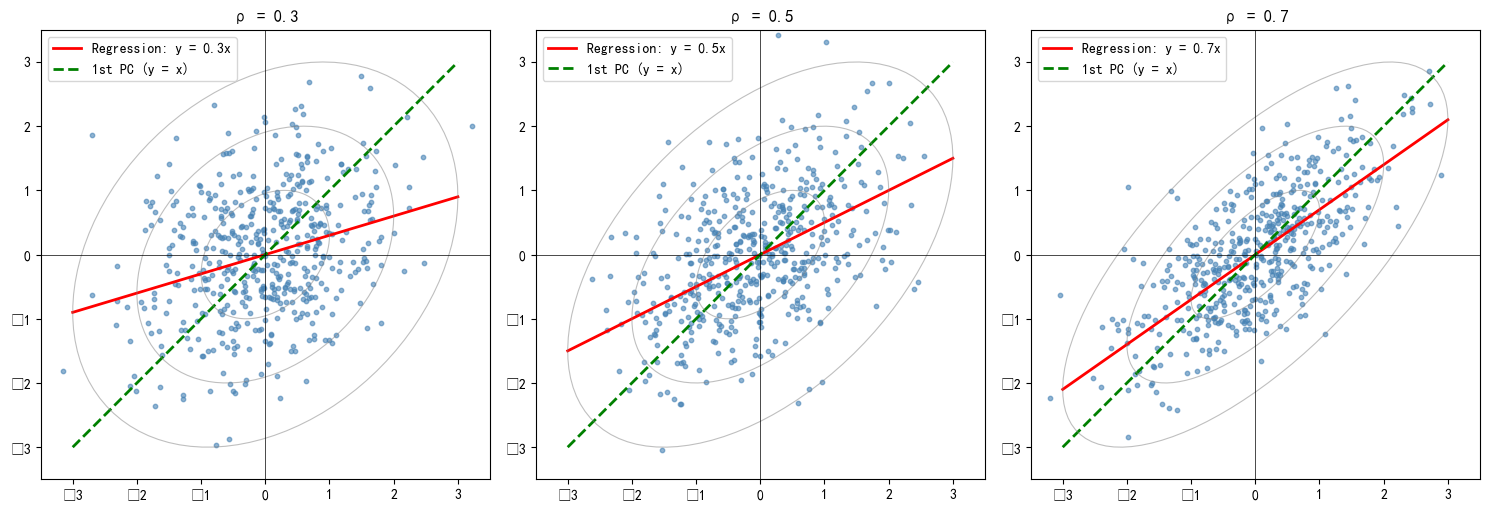
\includegraphics[width=\textwidth]{regression-principe-component.png}












\section*{The Chi-Squared Distribution: A Gentle Introduction}

\section{Introduction: Counting Deviations}

The Chi-Squared distribution ($\chi^2$) is the silent workhorse behind many statistical tests you encounter daily, from quality control in manufacturing to A/B testing in tech. At its heart, $\chi^2$ measures how much a set of observations \textit{deviates} from what you expect—whether those observations are coin flips, measurement errors, or distances in space. What makes it powerful is that it transforms these deviations into a single, interpretable number whose distribution is perfectly predictable.

\section{The Foundation: Squaring Standard Normals}

\subsection*{What is a Standard Normal?}

Before diving into $\chi^2$, we need the \textbf{Standard Normal Distribution}, denoted $Z \sim \mathcal{N}(0,1)$. This is the classic bell curve centered at 0 with a standard deviation of 1. It describes random fluctuations with no bias and unit spread—like the error in a perfectly calibrated measurement tool.

\subsection*{The Definition of Chi-Squared}

The $\chi^2$ distribution with \textbf{degrees of freedom} $k$ (written $\chi^2_k$) is defined as the sum of $k$ \textit{independent} squared standard normal variables:

\begin{equation}
    \boxed{X = Z_1^2 + Z_2^2 + \dots + Z_k^2 \quad \sim \quad \chi^2_k}
\end{equation}

Each $Z_i \sim \mathcal{N}(0,1)$ and all $Z_i$ are independent. The degrees of freedom $k$ count how many independent pieces of information are summed.

\section{Key Properties (Intuitively)}

- \textbf{Shape}: For $k=1$, it's heavily skewed. As $k$ grows, it becomes more symmetric and bell-shaped (by the Central Limit Theorem).
- \textbf{Mean}: $E[X] = k$. The average sum equals the number of terms.
- \textbf{Variance}: $\text{Var}(X) = 2k$. More terms mean more variability in the sum.
- \textbf{PDF}: $f(x; k) = \frac{1}{2^{k/2}\Gamma(k/2)} x^{k/2-1} e^{-x/2}$ for $x > 0$.

The key insight: $\chi^2$ is always non-negative because it's a sum of squares.

\section{Example 1: Random Walk Distance (Geometric Intuition)}

Imagine you take $k$ random steps in different directions. Each step's length in any dimension is a $Z_i \sim \mathcal{N}(0,1)$. The squared Euclidean distance from the origin is exactly the sum of these squared steps:

\begin{equation}
    \text{Distance}^2 = Z_1^2 + Z_2^2 + \dots + Z_k^2
\end{equation}

For a 2D random walk ($k=2$), the squared distance follows $\chi^2_2$. If you simulate this, you'll see most paths stay moderately close to the origin, but some wander far—exactly what $\chi^2_2$ predicts.

\section{Example 2: Estimating Variance (Statistical Core)}

Suppose you measure heights of $n$ people. The \textbf{sample variance} is:

\begin{equation}
    s^2 = \frac{1}{n-1}\sum_{i=1}^n (x_i - \bar{x})^2
\end{equation}

A remarkable result: If the true population is normal, the \textit{scaled} sum of squared deviations follows $\chi^2$:

\begin{equation}
    \boxed{(n-1)\frac{s^2}{\sigma^2} \sim \chi^2_{n-1}}
\end{equation}

\paragraph{Intuition:} While we sum $n$ squared deviations $(x_i - \bar{x})$, they are not independent—they must sum to zero. This constraint loses one degree of freedom, leaving $n-1$ independent pieces of information. This is why we divide by $n-1$ for an unbiased estimator.

\paragraph{Practical Use:} Build a 95\% confidence interval for the true variance $\sigma^2$:

\begin{equation}
    \text{CI} = \left[ \frac{(n-1)s^2}{\chi^2_{n-1,0.975}}, \frac{(n-1)s^2}{\chi^2_{n-1,0.025}} \right]
\end{equation}

Here $\chi^2_{k,\alpha}$ is the critical value cutting off $\alpha$ in the upper tail.

\section{Example 3: Testing a Fair Coin (Goodness-of-Fit)}

You flip a coin 100 times, getting 60 heads and 40 tails. Is the coin fair?

\paragraph{Expected vs. Observed:}
- Expected: 50 heads, 50 tails
- Observed: 60 heads, 40 tails

The $\chi^2$ \textbf{test statistic} quantifies the discrepancy:

\begin{equation}
    \chi^2 = \sum_{i=1}^{\text{categories}} \frac{(O_i - E_i)^2}{E_i}
\end{equation}

For our coin:
\begin{equation}
    \chi^2 = \frac{(60-50)^2}{50} + \frac{(40-50)^2}{50} = \frac{100}{50} + \frac{100}{50} = 4
\end{equation}

Degrees of freedom: $\text{categories} - 1 = 2 - 1 = 1$. Compare $\chi^2 = 4$ to $\chi^2_{1,0.05} \approx 3.84$. Since $4 > 3.84$, we reject fairness at the 5\% level—the coin likely is biased.

\paragraph{Why It Works (Rough Proof):} For large samples, $O_i \sim \mathcal{N}(E_i, E_i)$ approximately. Thus $(O_i - E_i)/\sqrt{E_i} \approx Z_i \sim \mathcal{N}(0,1)$, and the sum of their squares $\sum Z_i^2$ follows $\chi^2$. The constraint $\sum O_i = n$ loses one degree of freedom.

\section{Example 4: Does a Drug Work? (Test of Independence)}

A clinical trial tests a drug vs. placebo:

\begin{center}
\begin{tabular}{|c|cc|c|}
\hline
 & Recovered & Not Recovered & Total \\
\hline
Drug & 70 & 30 & 100 \\
Placebo & 50 & 50 & 100 \\
\hline
Total & 120 & 80 & 200 \\
\hline
\end{tabular}
\end{center}

Is recovery independent of treatment? Calculate expected counts assuming independence: $E_{11} = (100 \times 120)/200 = 60$.

The $\chi^2$ statistic sums over all 4 cells:
\begin{equation}
    \chi^2 = \sum_{i,j} \frac{(O_{ij} - E_{ij})^2}{E_{ij}} = \frac{(70-60)^2}{60} + \frac{(30-40)^2}{40} + \frac{(50-60)^2}{60} + \frac{(50-40)^2}{40} = 8.33
\end{equation}

Degrees of freedom: $(\text{rows}-1)(\text{columns}-1) = 1 \times 1 = 1$. Since $\chi^2_{1,0.05} = 3.84$ and $8.33 > 3.84$, we conclude recovery depends on treatment.

\section{Culmination: The Mahalanobis Distance Connection}

\subsection*{The Problem with Euclidean Distance}

Imagine measuring height ($h$) and weight ($w$) for adults. Heights vary by $\sim 4$ inches (SD), weights by $\sim 30$ pounds. If someone is 2 SDs tall and 2 SDs heavy, their Euclidean distance from average is $\sqrt{(2)^2 + (2)^2} = 2.83$. But this ignores that taller people tend to be heavier—variables are \textbf{correlated}. Mahalanobis distance fixes this.

\subsection*{Definition of Mahalanobis Distance}

For a random vector $\mathbf{Y} = (Y_1, \dots, Y_p)^T$ with mean $\boldsymbol{\mu}$ and covariance $\boldsymbol{\Sigma}$, the squared Mahalanobis distance for a point $\mathbf{y}$ is:

\begin{equation}
    D_M^2(\mathbf{y}) = (\mathbf{y} - \boldsymbol{\mu})^T \boldsymbol{\Sigma}^{-1} (\mathbf{y} - \boldsymbol{\mu})
\end{equation}

\subsection*{Why It's Chi-Squared: The Algebraic Magic}

Assume $\mathbf{Y} \sim \mathcal{N}_p(\boldsymbol{\mu}, \boldsymbol{\Sigma})$. The key step is \textbf{decorrelation} via the transformation:

\begin{equation}
    \mathbf{Z} = \boldsymbol{\Sigma}^{-1/2}(\mathbf{Y} - \boldsymbol{\mu})
\end{equation}

\paragraph{What is $\boldsymbol{\Sigma}^{-1/2}$?} It's the matrix square root of $\boldsymbol{\Sigma}^{-1}$. Geometrically, it:
1. \textbf{Centers} the data by subtracting $\boldsymbol{\mu}$.
2. \textbf{Rotates} to align with principal components (undoing correlation).
3. \textbf{Scales} each component to unit variance.

\paragraph{Distribution of $\mathbf{Z}$:}
- $\mathbf{Z}$ is multivariate normal because it's a linear transformation of a normal vector.
- $E[\mathbf{Z}] = \mathbf{0}$.
- $\text{Cov}(\mathbf{Z}) = \boldsymbol{\Sigma}^{-1/2} \boldsymbol{\Sigma} \boldsymbol{\Sigma}^{-1/2} = \mathbf{I}_p$ (the identity matrix).

Thus, $\mathbf{Z} \sim \mathcal{N}_p(\mathbf{0}, \mathbf{I}_p)$. Critically, its components $Z_1, \dots, Z_p$ are \textbf{independent} standard normals!

\paragraph{The Chi-Squared Emergence:}
Now compute the squared Mahalanobis distance using $\mathbf{Z}$:
\begin{align*}
    D_M^2(\mathbf{y}) &= (\mathbf{y} - \boldsymbol{\mu})^T \boldsymbol{\Sigma}^{-1} (\mathbf{y} - \boldsymbol{\mu}) \\
    &= (\mathbf{y} - \boldsymbol{\mu})^T \boldsymbol{\Sigma}^{-1/2}\boldsymbol{\Sigma}^{-1/2} (\mathbf{y} - \boldsymbol{\mu}) \\
    &= \big[\boldsymbol{\Sigma}^{-1/2}(\mathbf{y} - \boldsymbol{\mu})\big]^T \big[\boldsymbol{\Sigma}^{-1/2}(\mathbf{y} - \boldsymbol{\mu})\big] \\
    &= \mathbf{z}^T\mathbf{z} = \sum_{j=1}^p z_j^2
\end{align*}

Since each $z_j \sim \mathcal{N}(0,1)$ and independent, by the \textbf{definition} of $\chi^2$:

\begin{equation}
    \boxed{D_M^2(\mathbf{y}) \sim \chi^2_p}
\end{equation}

\subsection*{Practical Example: Outlier Detection in 2D}

Suppose heights ($H$) and weights ($W$) have:
\[
\boldsymbol{\mu} = (68\,\text{in}, 150\,\text{lb}), \quad \boldsymbol{\Sigma} = \begin{pmatrix} 16 & 60 \\ 60 & 900 \end{pmatrix}
\]

A person is $(72\,\text{in}, 180\,\text{lb})$. The Mahalanobis distance is:
\[
D_M^2 = (4, 30) \begin{pmatrix} 16 & 60 \\ 60 & 900 \end{pmatrix}^{-1} \begin{pmatrix} 4 \\ 30 \end{pmatrix} = 2.5
\]

Since $D_M^2 = 2.5 < \chi^2_{2,0.95} = 5.99$, this person is within the 95\% confidence ellipse—\textbf{not an outlier}.

Now consider $(80\,\text{in}, 160\,\text{lb})$ (tall but not proportionally heavy):
\[
D_M^2 = (12, 10) \boldsymbol{\Sigma}^{-1} \begin{pmatrix} 12 \\ 10 \end{pmatrix} = 8.2
\]

Since $8.2 > 5.99$, this point lies outside the ellipse—an outlier! Euclidean distance would miss this because it ignores the height-weight correlation.

\section{Conclusion: The Power of Chi-Squared}

The Chi-Squared distribution is not just a formula—it's a \textbf{lens} for viewing variability. Whether counting coin flips, measuring distances, or detecting outliers, $\chi^2$ quantifies how much random deviation is "too much." Its marriage with Mahalanobis distance creates a robust tool for navigating high-dimensional, correlated data, turning complex geometries into simple probabilistic statements. The next time you see an ellipse on a scatterplot, remember: its boundary is a contour of constant Chi-Squared distance, separating the normal from the anomalous.










\section*{The F-Test for R²: Connecting Variance Explained to Statistical Significance}

\section{What is the F-Test for R²?}

The \textbf{F-test for R²} is a formal hypothesis test that answers: \textit{Does our regression model explain a statistically significant portion of the variance in the outcome variable?} It tests the null hypothesis:

\begin{align*}
    H_0 &: R^2 = 0 \quad \text{(the model explains nothing; all slope coefficients } \beta_1 = \beta_2 = \dots = \beta_k = 0) \\
    H_a &: R^2 > 0 \quad \text{(at least one predictor is useful)}
\end{align*}

The test statistic is computed from your regression output and follows an \textbf{F-distribution} under the null hypothesis.

\section{The Formula: Where R² Meets F}

For a linear regression with \textbf{k} predictors and \textbf{n} observations:

\begin{equation}
    F = \frac{R^2/k}{(1 - R^2)/(n - k - 1)}
\end{equation}

This is identical to the \textbf{overall F-statistic} reported in regression ANOVA tables. A large F-value (relative to the critical value from $F_{k, n-k-1}$) leads to rejecting $H_0$.

\section{Origin: The Sum of Squares Decomposition}

The F-test emerges from the \textbf{ANOVA decomposition} of total variance:

\begin{equation}
    SST = SSR + SSE
\end{equation}

Where:
\begin{itemize}
    \item \textbf{SST} = Total Sum of Squares $= \sum_{i=1}^n (y_i - \bar{y})^2$ (total variation in y)
    \item \textbf{SSR} = Regression Sum of Squares $= \sum_{i=1}^n (\hat{y}_i - \bar{y})^2$ (variation explained by model)
    \item \textbf{SSE} = Error Sum of Squares $= \sum_{i=1}^n (y_i - \hat{y}_i)^2$ (unexplained variation)
\end{itemize}

Recall that: $R^2 = \dfrac{SSR}{SST} = 1 - \dfrac{SSE}{SST}$

\section{Derivation: From Sums of Squares to F-Statistic}

Under the null hypothesis (all $\beta_j = 0$), with the assumption of normally distributed errors $\varepsilon_i \sim \mathcal{N}(0, \sigma^2)$, the following distributions hold:

\begin{enumerate}
    \item $\dfrac{SSE}{\sigma^2} \sim \chi^2_{n-k-1}$ \quad (chi-squared with $n-k-1$ degrees of freedom)
    \item $\dfrac{SSR}{\sigma^2} \sim \chi^2_{k}$ \quad (chi-squared with $k$ degrees of freedom) \textbf{if $H_0$ is true}
    \item $SSR$ and $SSE$ are independent
\end{enumerate}

\subsection*{The Key Insight}

The F-distribution is defined as the ratio of two independent chi-squared variables, each divided by their degrees of freedom:

\begin{equation}
    F = \frac{(\chi^2_{df_1} / df_1)}{(\chi^2_{df_2} / df_2)}
\end{equation}

\subsection*{Constructing the Test Statistic}

\begin{align*}
    F &= \frac{(SSR/\sigma^2)/k}{(SSE/\sigma^2)/(n-k-1)} \\
      &= \frac{SSR/k}{SSE/(n-k-1)} \quad \text{($\sigma^2$ cancels)} \\
      &= \frac{(SSR/SST)/k}{(SSE/SST)/(n-k-1)} \quad \text{(divide numerator and denominator by SST)} \\
      &= \frac{R^2/k}{(1 - R^2)/(n - k - 1)}
\end{align*}

This is the bridge between the sums of squares (foundational theory) and $R^2$ (practical measure).

\section{Interpretation: What the F-Test Tells You}

\begin{itemize}
    \item \textbf{Large F} (e.g., $F > F_{\text{critical}}$): Your model explains significantly more variance than expected by chance. Reject $H_0$.
    \item \textbf{Small F} (e.g., $F \approx 1$): The explained variance is comparable to the unexplained variance per degree of freedom. Fail to reject $H_0$.
\end{itemize}

The p-value from the F-test is exactly the probability of observing an $R^2$ as large as you did if the true $R^2$ were zero.

\section{Special Case: Simple Linear Regression ($k = 1$)}

For one predictor, the F-test for $R^2$ is \textbf{equivalent to the t-test for the slope}:

\begin{equation}
    F = t_\beta^2 = \frac{R^2}{(1 - R^2)/(n - 2)}
\end{equation}

This makes sense: if there's only one slope, testing ``is $R^2 > 0$?'' is the same as testing ``is $\beta_1 \neq 0$?''

\section{Connection to Partial F-Tests}

The same logic extends to comparing \textbf{nested models}. Want to test if adding 2 new predictors significantly improves $R^2$?

\begin{equation}
    F = \frac{(R^2_{\text{full}} - R^2_{\text{reduced}})/2}{(1 - R^2_{\text{full}})/(n - k_{\text{full}} - 1)}
\end{equation}

This tests the null that the new predictors' coefficients are both zero.

\section{Historical Origin: R.A. Fisher's Breakthrough (1920s)}

The F-test was developed by \textbf{Sir Ronald Fisher} in the 1920s as part of his work on \textbf{Analysis of Variance (ANOVA)}. Fisher realized that by comparing the ratio of explained to unexplained variance (properly scaled by degrees of freedom), he could develop a general method for testing hypotheses in linear models. The distribution of this ratio—now called the \textbf{F-distribution}—was named in his honor. The connection to $R^2$ was a natural consequence of Fisher's variance decomposition framework.

\section{Summary: The F-Test for R² in Practice}

\begin{enumerate}
    \item \textbf{Compute $R^2$} from your regression.
    \item \textbf{Plug into the formula}: $F = \dfrac{R^2/k}{(1-R^2)/(n-k-1)}$
    \item \textbf{Compare to F-distribution}: Use degrees of freedom $(k, n-k-1)$.
    \item \textbf{Make a decision}: Reject $H_0$ if \texttt{p-value} $< \alpha$.
\end{enumerate}

The test is powerful because it leverages the elegant theory of quadratic forms and chi-squared distributions, providing a rigorous bridge between descriptive statistics ($R^2$) and inferential statistics (hypothesis testing).

\end{document}

